%%%%%%%%%%%%%%%%%%%%%%%%%%%%%%%%%%%%%%%%%%%%%%%%%%%%%%%%%%%%%%%%%%%%%%%
%% Vorlage f�r Abschlussarbeiten                                     %%
%%-------------------------------------------------------------------%%
%% Datei:        basics.tex                                         %%
%% Beschreibung: Grundlagenteil welcher verwendete Hard-   %%
%%               und Software n�her beschreibt.                            %%
%% Autor: 			 Stefan Herrmann                                     %%
%% Datum:        04.12.2012                                          %%
%% Version:      1.0.1                                               %%
%%%%%%%%%%%%%%%%%%%%%%%%%%%%%%%%%%%%%%%%%%%%%%%%%%%%%%%%%%%%%%%%%%%%%%%

\chapter{Grundlagen}
\index{Grundlagen} %% Eintrag im Stichwortverzeichnis
In diesem Kapitel wird auf die Grundlagen, zu verwendeten Verfahren sowie zu verwendeten neuronalen Netzen, eingegangen. Dies soll die notwendigen Informationen, zur gesamten Arbeit und speziell f�r die Ausf�hrungen im dritten und vierten Kapitel, bereitstellen. Hierbei werden nur die, f�r das Verst�ndnis der Arbeit, wesentlichen Komponenten beschrieben.

\section{Eulerian Magnification}
\index{Eulerian Magnification}
Die menschliche F�higkeit, �nderungen in der Umgebung visuell wahrzunehmen, hat eine beschr�nkte r�umlich-zeitliche Empfindlichkeit. Dies hat als Konsequenz, dass �nderungen die Au�erhalb dieses Empfindlichkeitsbereiches liegen, nicht von Menschen wahrgenommen werden k�nnen. Viele dieser subtilen �nderungen, die au�erhalb der menschlichen Wahrnehmung liegen, beinhalten jedoch Informationen die von Interesse sein k�nnen. Zum Beispiel �ndert sich, durch die zeitlich unterschiedliche Durchblutung, die Hautfarbe im Gesicht eines Menschen �ber die Zeit. Diese nicht wahrnehmbare �nderung, wenn sichtbar gemacht, kann zum Beispiel f�r die visuelle Messung der Pulsfrequenz einer Person genutzt werden.\cite{Philips,Poh:10,Verkruysse:08}
Um diese Informationen in Videos sichtbar zu machen, gibt es mehrere Ans�tze. Neben der ''Lagrangian Motion Magnification'', welche mit optischem Fluss arbeitet, gibt es die ''Eulerian Video Magnification''. Letztere Methode kombiniert r�umliche und zeitliche Verarbeitung, um die subtilen zeitlichen �nderungen in einem Video hervorzuheben. Im Gegensatz zur Verwendung von optischem Fluss zur Sch�tzung von �nderungen, ist dieser Ansatz nicht rechenintensiv und somit auch f�r Echtzeitanwendungen geeignet.(todo Zitat eulerianmagnificationpaper)

\subsection{Ablauf der Videoverarbeitung}
\index{Ablauf der Videoverarbeitung}
 Im ersten Schritt, wird das Video in unterschiedliche Ortsfrequenzb�nder zerlegt. Diese Zerlegung wird durch den Aufbau von einer Bildpyramide erreicht. Als n�chstes werden diese Ortsfrequenzb�nder im Zeitbereich verarbeitet. Hierzu wird angenommen, dass die Zeitfolge mit dem Wert eines Pixels, in einem Frequenzband, korresponidert und es wird ein Bandpass angewandt. Hiermit sollen die Frequenzb�nder, die von Interesse sind, extrahiert werden. Das extrahierte Signal wird mit einem Verst�rkungsfaktor multipliziert und auf das Ausgangssignal addiert. Im letzten Schritt wird aus der resultierenden Bildpyramide, dass Zielvideo rekonstruiert. Der Prozess, der ''Eulerian Video Magnification'', ist nochmal in Abbildung 1(todo Zitat eulerianmagnificationpaper) visuell dargestellt.

\begin{figure}
	\centering
		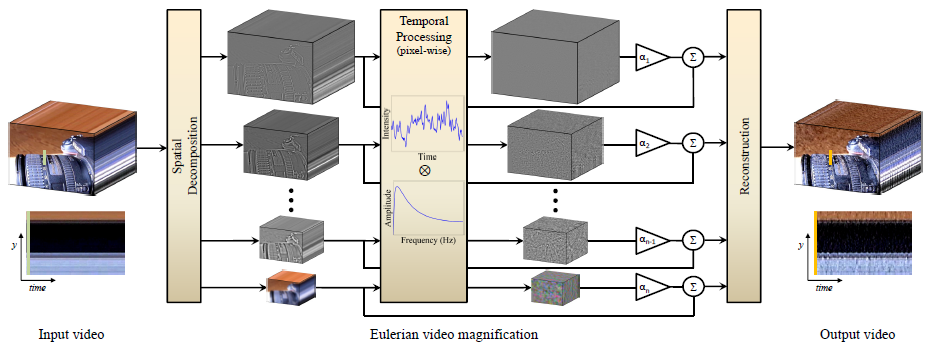
\includegraphics[width=1.0\textwidth]{images/basics/ProcessEulerianVideoMagnification.png}
	\caption{Prozess ''Eulerian Video Magnification''}
	\label{fig:Prozess ''Eulerian Video Magnification''}
\end{figure}

\subsection{Bildpyramiden}
Bildpyramiden sind Mehrgitterdarstellungen von Bildern, welche verwendet werden, um Bilder auf verschiedenen Skalen zu analysieren und zu verarbeiten. Um so eine Darstellung eines Bildes zu erhalten, wird das Bild iterativ Gefiltert und Unterabgetastet. Das Ergebnis ist eine Pyramide von Bildern, bei der jedes Bild eine andere Skala repr�sentiert. Hierbei ist das verwendete Filter ein Gl�ttungsfilter, um eine Verletzung der Abtastbedingung, bei der Verarbeitung der n�chsten Stufe, zu verhindern. 

\subsubsection*{Gau�-Pyramide}

\subsubsection*{Laplace-Pyramide}

\subsubsection*{Steuerbare Pyramide}


\subsection{Farbverst�rkung}

\subsection{Bewegungsverst�rkung}


\section{CNN}


\subsection{1D-CNN}


\subsection{3D-CNN}